%%%%%%%%%%%%%%%%%%%%%%%%%%%%%%%%%%%%%%%%%
% University Assignment Title Page 
% LaTeX Template
% Version 1.0 (27/12/12)
%
% This template has been downloaded from:
% http://www.LaTeXTemplates.com
%
% Original author:
% WikiBooks (http://en.wikibooks.org/wiki/LaTeX/Title_Creation)
%
% License:
% CC BY-NC-SA 3.0 (http://creativecommons.org/licenses/by-nc-sa/3.0/)
% 
% Instructions for using this template:
% This title page is capable of being compiled as is. This is not useful for 
% including it in another document. To do this, you have two options: 
%
% 1) Copy/paste everything between \begin{document} and \end{document} 
% starting at \begin{titlepage} and paste this into another LaTeX file where you 
% want your title page.
% OR
% 2) Remove everything outside the \begin{titlepage} and \end{titlepage} and 
% move this file to the same directory as the LaTeX file you wish to add it to. 
% Then add \input{./title_page_1.tex} to your LaTeX file where you want your
% title page.
%
%%%%%%%%%%%%%%%%%%%%%%%%%%%%%%%%%%%%%%%%%
%\title{Title page with logo}
%----------------------------------------------------------------------------------------
%	PACKAGES AND OTHER DOCUMENT CONFIGURATIONS
%----------------------------------------------------------------------------------------

\documentclass[12pt]{article}
\usepackage[english]{babel}
\usepackage[utf8x]{inputenc}
\usepackage{amsmath}
\usepackage{graphicx}
\usepackage[colorinlistoftodos]{todonotes}
\usepackage{hyperref}

\begin{document}

\begin{titlepage}

\newcommand{\HRule}{\rule{\linewidth}{0.5mm}} % Defines a new command for the horizontal lines, change thickness here

\center % Center everything on the page

%----------------------------------------------------------------------------------------
%	LOGO SECTION
%----------------------------------------------------------------------------------------


\includegraphics{logo.png}\\ % Include a department/university logo - this will require the graphicx package
 
%----------------------------------------------------------------------------------------
 
%----------------------------------------------------------------------------------------
%	HEADING SECTIONS
%----------------------------------------------------------------------------------------


\textsc{\Large Cloud Computing}\\[0.5cm] % Major heading such as course name
\textsc{\large Bachelor of Science (Hons) Applied Computing }\\[0.5cm] % Minor heading such as course title

%----------------------------------------------------------------------------------------
%	TITLE SECTION
%----------------------------------------------------------------------------------------

\HRule \\[0.4cm]
{ \huge \bfseries iSCSI Storage Exercise}\\[0.4cm] % Title of your document
\HRule \\[1.5cm]
 
%----------------------------------------------------------------------------------------
%	AUTHOR SECTION
%----------------------------------------------------------------------------------------



% If you don't want a supervisor, uncomment the two lines below and remove the section above

\Large Ciaran \textsc{Roche} - 20037160\\[3cm] % Your name

%----------------------------------------------------------------------------------------
%	DATE SECTION
%----------------------------------------------------------------------------------------

{\large \today}\\[1cm] % Date, change the \today to a set date if you want to be precise


\vfill % Fill the rest of the page with whitespace

\end{titlepage}


\section{Introduction}

Based on lab exercises completed a number of tasks where under taken. This document reports the steps taken in the tasks along with some explanation behind the tasks. These exercises where completed as part of the EMC Cloud Infrastructure and Services exercises. These exercises show some of the principles and concepts of vitalization and cloud infrastructure technologies.
These exercises included hands on experience with using VMware vSphere. vSphere is a suite of virtualization application that include ESXi and vCenter Server. vSphere uses virtualization to do a number of tasks, like run multiple operating systems on a single physical machine simultaneously. Reclaim idle resources and balance workloads across multiple physical machines and also work around hardware failures and scheduled maintenance.

\section{Tasks}
The following tasks where completed in this report.
\begin{enumerate}
    \item Create a new iSCSI volume on NAS02. The Volume Manager should be RAID-Z
    \item Create an iSCSI target as Lab 2, choose a file extent or device extent with an explanation of the difference betweem the two and why it was chosen.
    \item Security/Authentication to be configured to enable authentication.
    \item Create a new iSCSI datastore on the ESXi02 host. Outline the size of the datastore.
    \item Create a new iSCSI initiator on ESXi02 by adding an iSCSI software adapter.
    \item Create a new iSCSI datastore which is accessible from both ESXi hosts.
    \item Demonstrate that the iSCSI LUNs are available to the Ubuntu client and also the CentOS virtual machine
    \item Virtual Switches should not be reconfigured.
\end{enumerate}

\section{Topology}
The topology throughout this exercise:

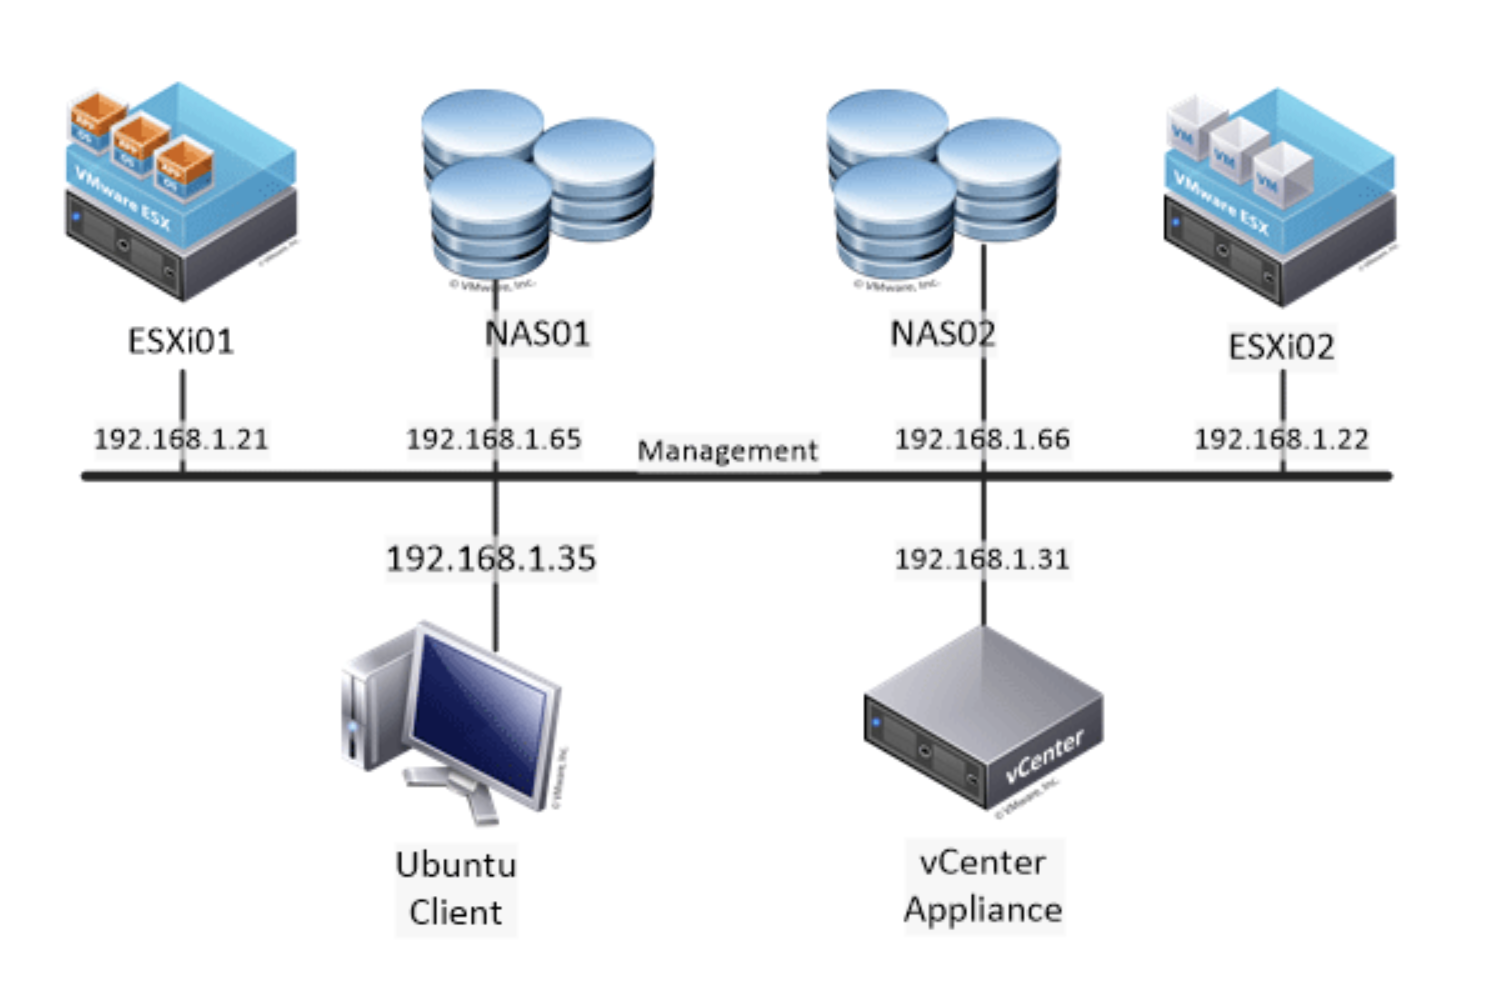
\includegraphics[width=\textwidth]{topology.png}
\section{Tasks}
First task will outline the creation of an iSCSI volume on NAS02. The Volume Manager will be RAID-Z.

iSCSI (Internet Small Computer System Interface) is a transport layer protocol which outlines how SCSI packets are to be transported over a TCP/IP network. These packets are sent between an iSCSI initiator on a server to a iSCSI target on a storage device. The iSCSI protocol encapsulates SCSI commands and packages the data for the TCP/IP layer. These packets are sent over the network using a point to point connection \cite{iscsi}. There will be detailed steps on setting up an iSCSI initiator later in the report. 

To start once the pod was successfully loaded, I signed into the Ubuntu client and opened Firefox. This presents me with the EMC CIS Web Home Page which allows me to log into either NAS storage or my VCenter Appliance. From here I select NAS02
\newline
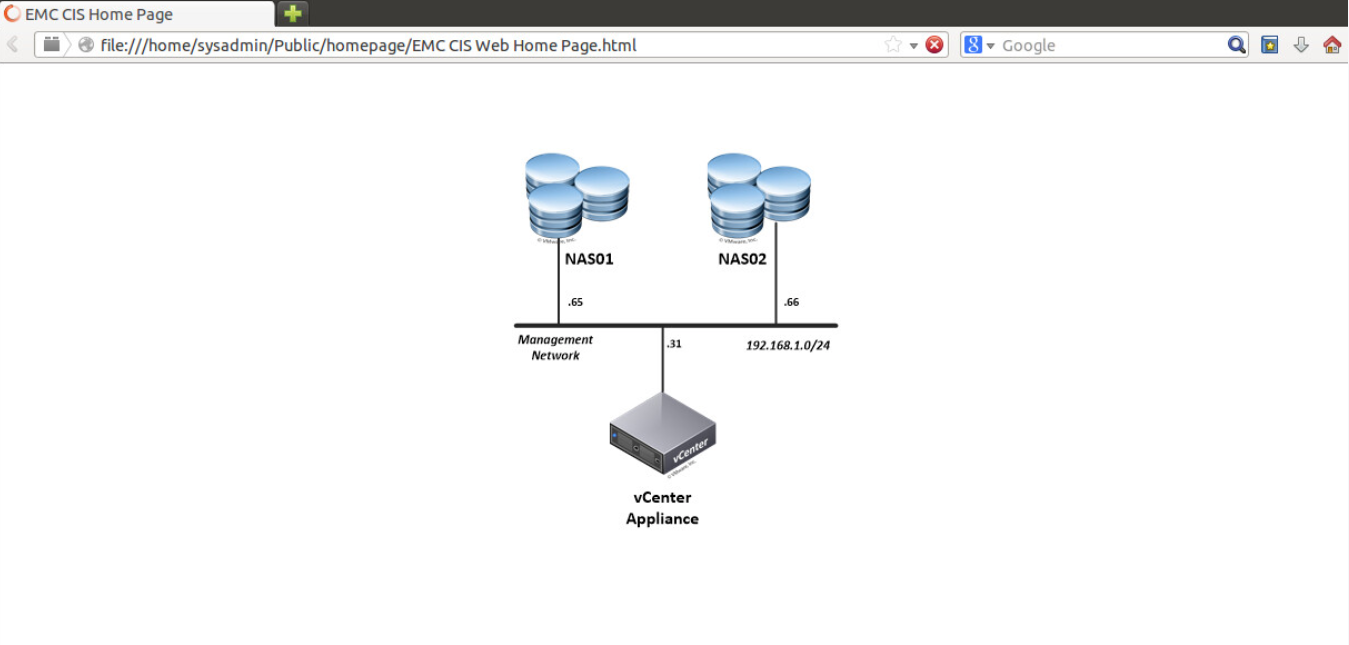
\includegraphics[width=\textwidth]{1.png}
Navigate to services and ensure iSCSI is turned on.
\newline
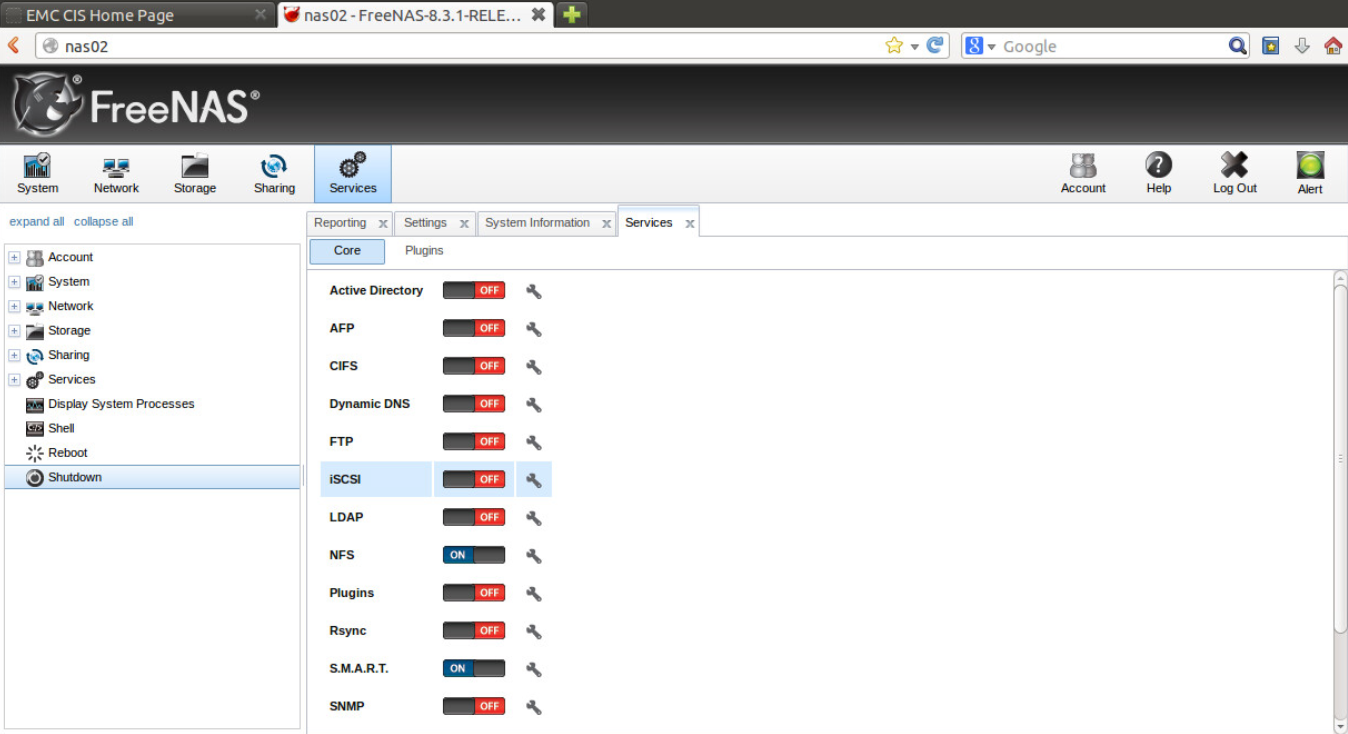
\includegraphics[width=\textwidth]{2.png}
\newpage
With iSCSI turned on the next step is to navigate to Storage-Active Volumes. From here I can do things like import a volume, view the disks, or even just get an overview of volumes. What I need to do is select the Volume Manager 
\newline
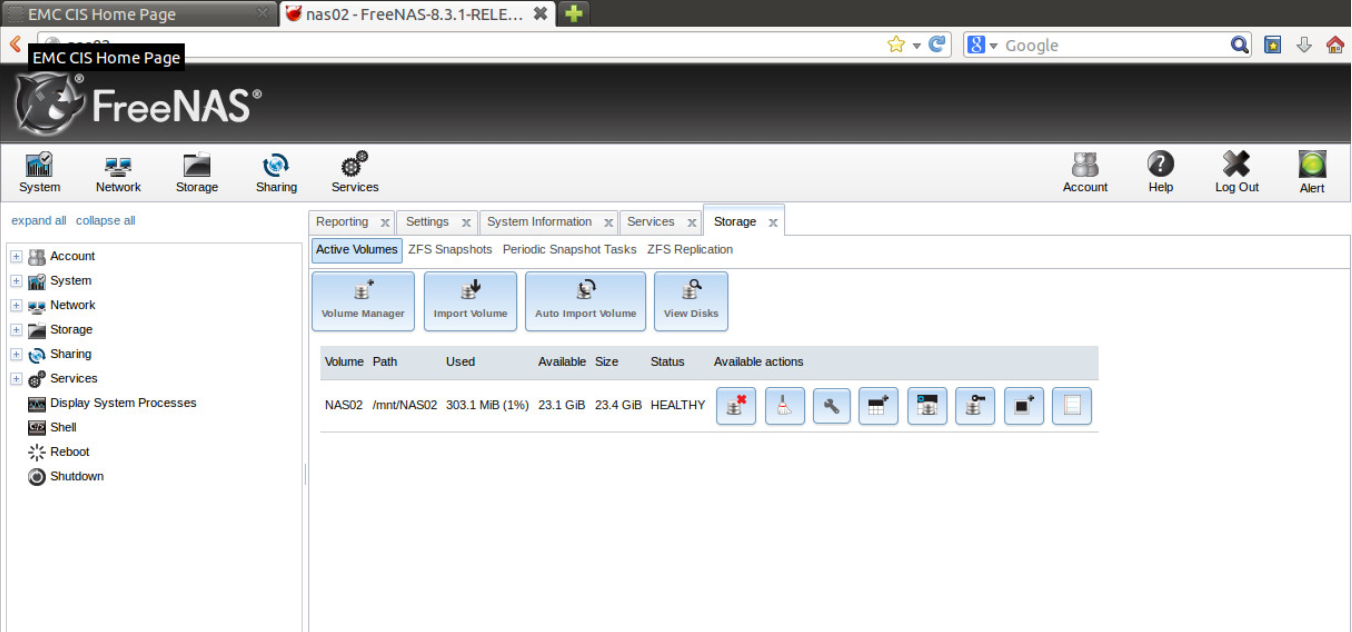
\includegraphics[width=\textwidth]{3.png}
\newpage
Once in the Volume Manager I complete the following settings to add a new volume:
\begin{center}
\begin{tabular}{ |c|c| } 
 \hline
 Name & RAIDZ \\ 
 Member Disks & da11, da12, da13\\ 
 Filesystem Type & ZFS \\ 
 Group Type & RAID-Z \\
 \hline
\end{tabular}
\end{center}
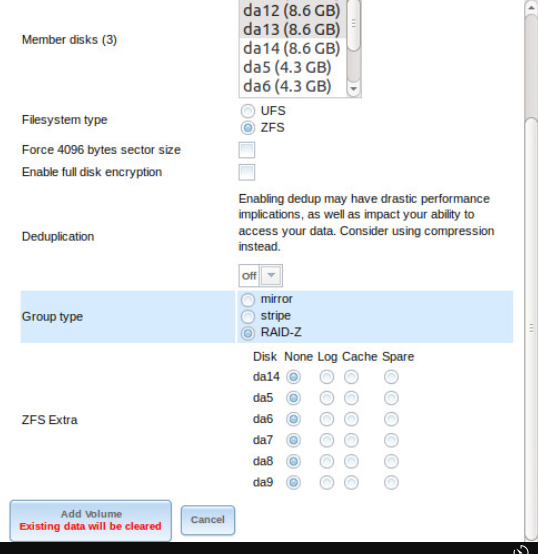
\includegraphics[width=\textwidth]{4.png}
\newpage
After clicking Add Volume I am returned to Active Volumes and as can be seen from the screen below the new volume has been added to the overview.
\newline
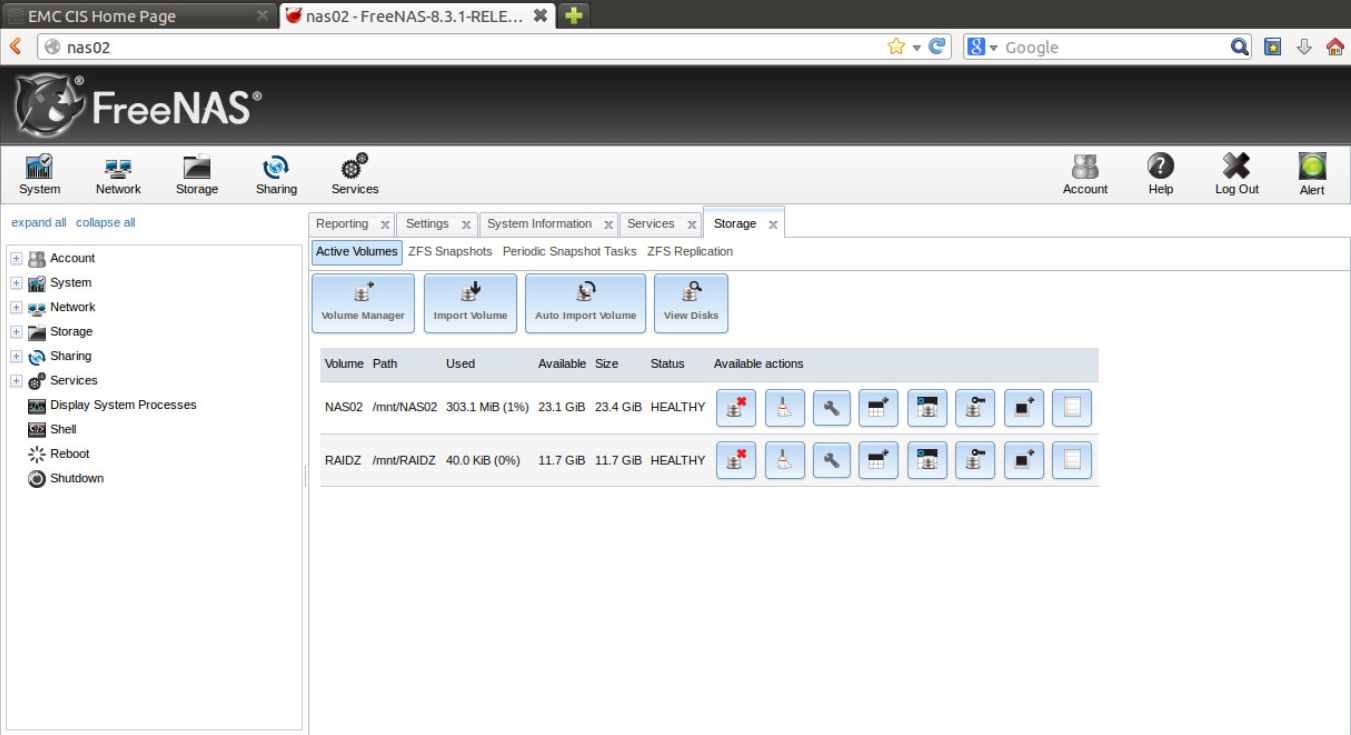
\includegraphics[width=\textwidth]{5.png}
\newline
RAID-Z is similar to RAID-5 in that disks are maintained in a way that loss of any one disk would not result in data loss. It has a distributed parity which means all disks participate equally in the reads. Unlike RAID-5, RAID-Z splits data blocks across all disks. Parity is often a bitwise XOR of the blocks in a row \cite{raidz}


The next task will create an iSCSI target as described in Lab 2, along with provide an explanation of the difference between file extent and device extent.
To understand the difference between a file extent and a device extent we need to understand what an extent is first. To put in layman's terms and extent is a partition on a storage volume or LUN \cite{extent}. A LUN (Logical Unit Number) is a unique identifier for designating an individual or collection of physical or virtual storage devices \cite{lun}.
To break down my understanding of the difference of file and device extents if we imagine our partition as a tree of nodes, a device extent would look at the entire tree where as a file extent would only look at a single node \cite{extent2}.

As can be seen from the screenshot below, I am on the FreeNas dashboard and have navigated to Storage/Active Volumes, I have an new volume created called iSCSI, with the path /mnt/iSCSI
\\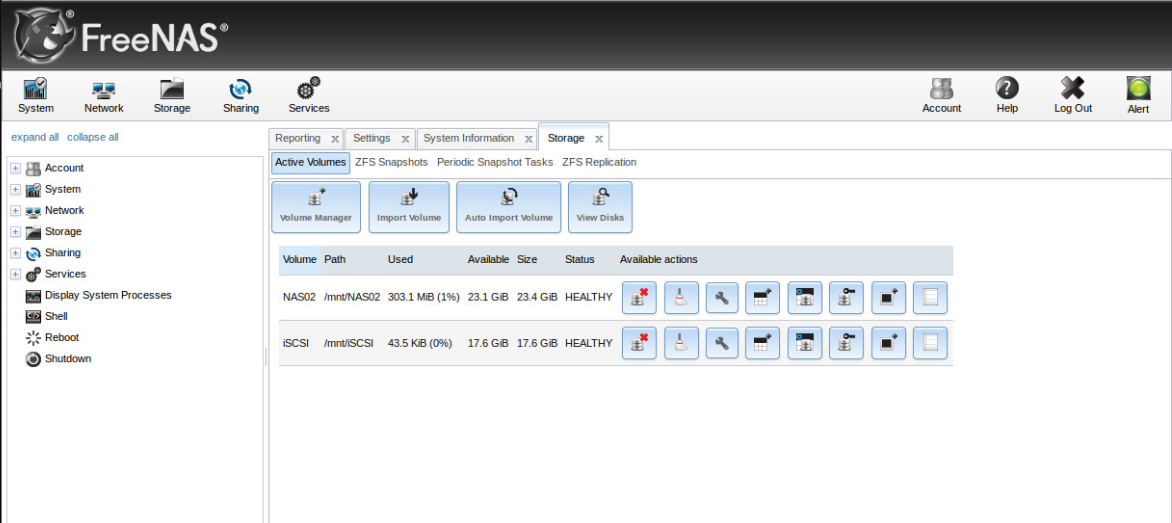
\includegraphics[width=\textwidth]{8.png}
\\ The next step is navigate to services and turn iSCSI on.
\\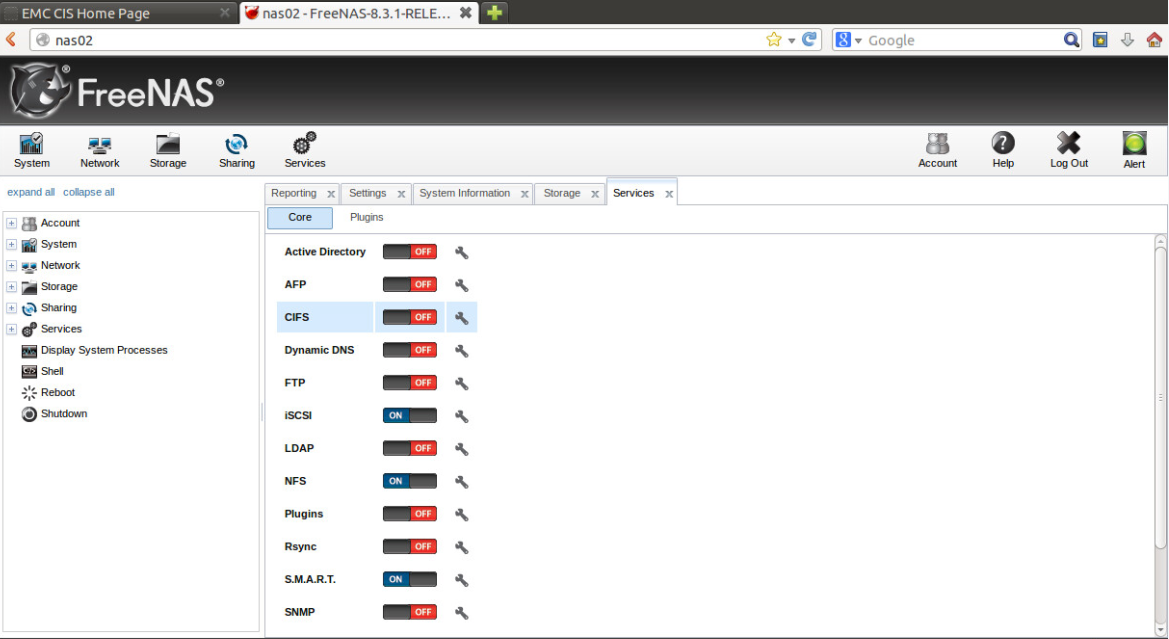
\includegraphics[width=\textwidth]{7.png}
\\ With iSCSI turned on I select iSCSI settings and navigate to Targets. Ahead of this step I have configured a default portal group and default initiator group. With the preconfigured groups I enter the following into the new target configuration:
\begin{center}
\begin{tabular}{ |c|c| } 
 \hline
 Target Name & iscsi01 \\ 
 Portal Group ID & 1 (Default)\\ 
 Initiator Group ID & 1 (Default) \\ 
 Auth Method & None \\
 \hline
\end{tabular}
\end{center}
All the rest of the configuration remain as default.
\\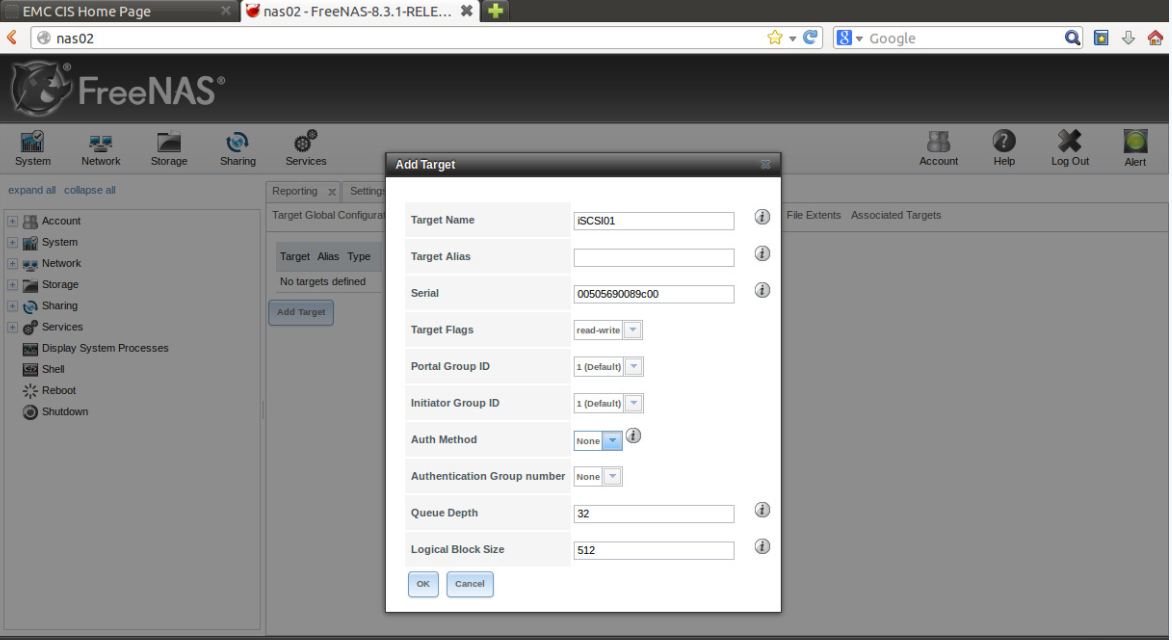
\includegraphics[width=\textwidth]{6.png}
The next step is to create an extent, for this exercise I chose a file extent, so to create this I selected file extent from the tab menu, and entered the following settings:
\begin{center}
\begin{tabular}{ |c|c| } 
 \hline
 Extent Name & iscsiext \\ 
 Path to the extent & /mnt/iSCSI/iscsiext\\ 
 Extent Size & 5 GB \\ 
 \hline
\end{tabular}
\end{center}
The rest of the configuration remained as default.
\\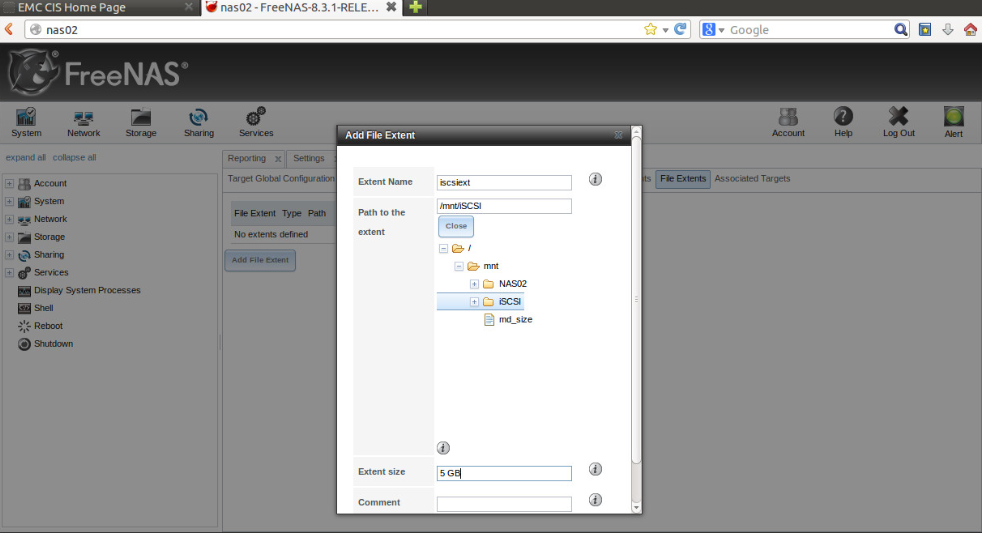
\includegraphics[width=\textwidth]{9.png}
What I have done here is created an extent file the size of 5 GB within the iSCSI volume which I created in Task 1.
\\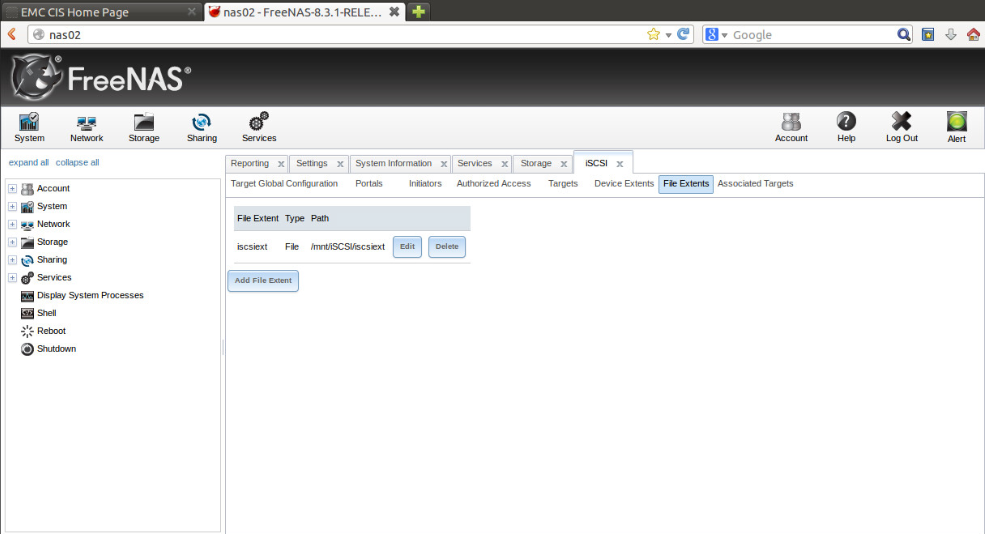
\includegraphics[width=\textwidth]{10.png}
The next step was to add the extent to the target, this was done by selecting Associated Targets from the tab menu, and setting the target and extent to that which I just created
\\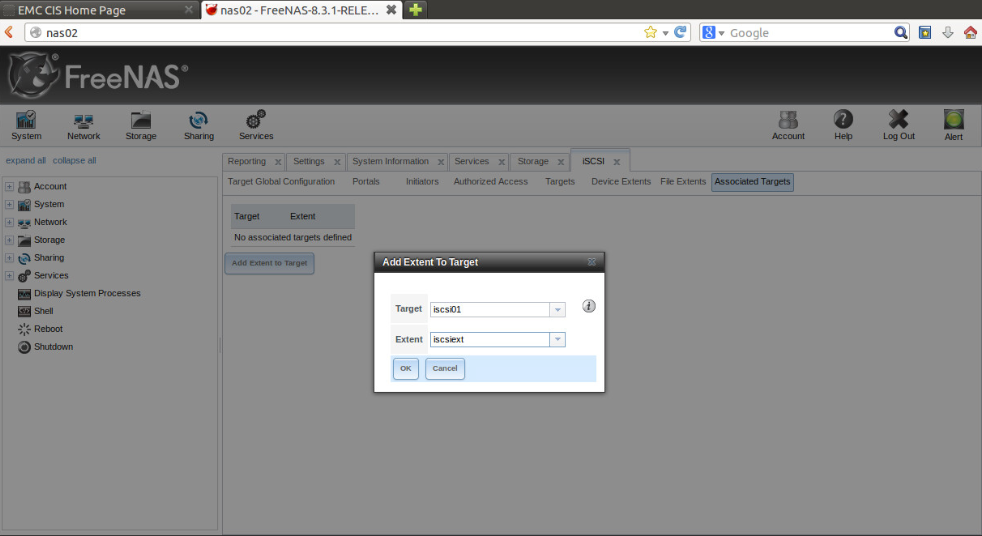
\includegraphics[width=\textwidth]{11.png}
To sum up what has been done to date, an iSCSI volume was created on nas02, I then set up an iSCSI target to which I also created an extent within the volume. Finally I associated the target with the extent. This allows the extent be accessible to multiple initiators is needs be. 


Moving on I will configure authentication on the iSCSI target which was created in the previous task.
There is a number of iSCSI terminology that needs to be understood before proceeding with the configuration of the authentication. 
\\\textbf{CHAP :} is an authentication method that uses both a shared secret and a three-way authentication to grant access to a storage device.
\\\textbf{Mutual CHAP : } In CHAP the authentication takes place on the initiator, where as mutual CHAP both devices authenticate each other \cite{CHAP}

To enable authentication on a target I first navigate back to FreeNAS and to Services, select iSCSI settings and then Authorized Access, here I create a User which can be seen in the screen shot below.
\\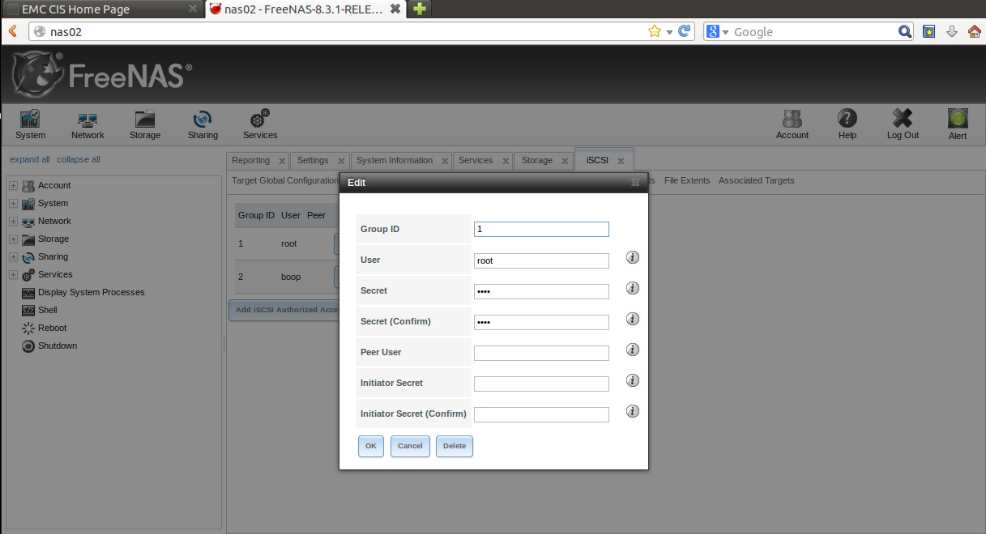
\includegraphics[width=\textwidth]{12.png}
With a user created I go targets and select edit on my created iscsi01 target. Here I select the Auth Method, which is explained above, I select CHAP. Finally I need to set the Authentication Group number, I do this my selecting the id value to the user which was created in the previous step.
\\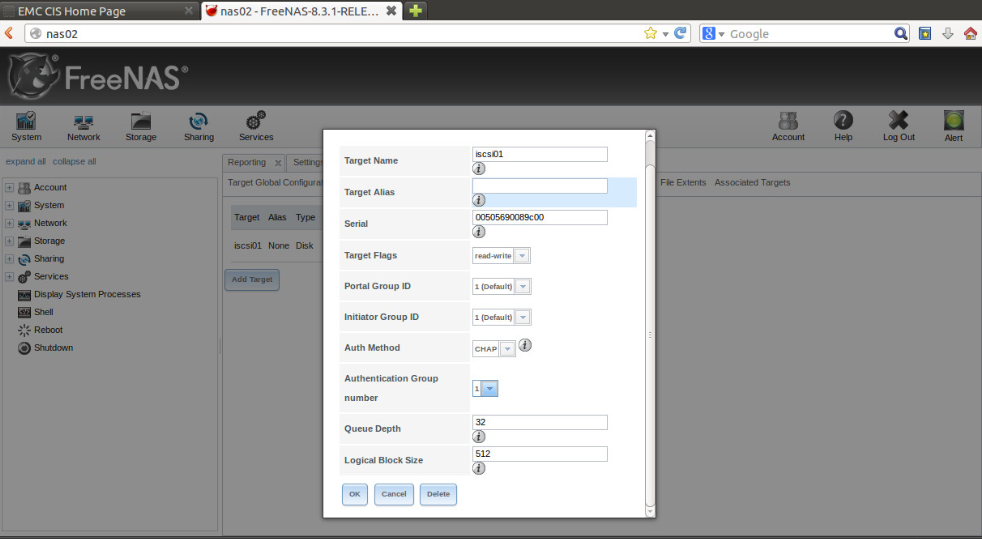
\includegraphics[width=\textwidth]{13.png}
And that is it, I have now created a user and set CHAP authentication on my target.

With a volume set up on Nas02 and configured the following steps will create an initiator and datastore which is accessible from both ESXi hosts. The first step is to open a terminal on the ubuntu client and run the discovery command to see available targets.
\\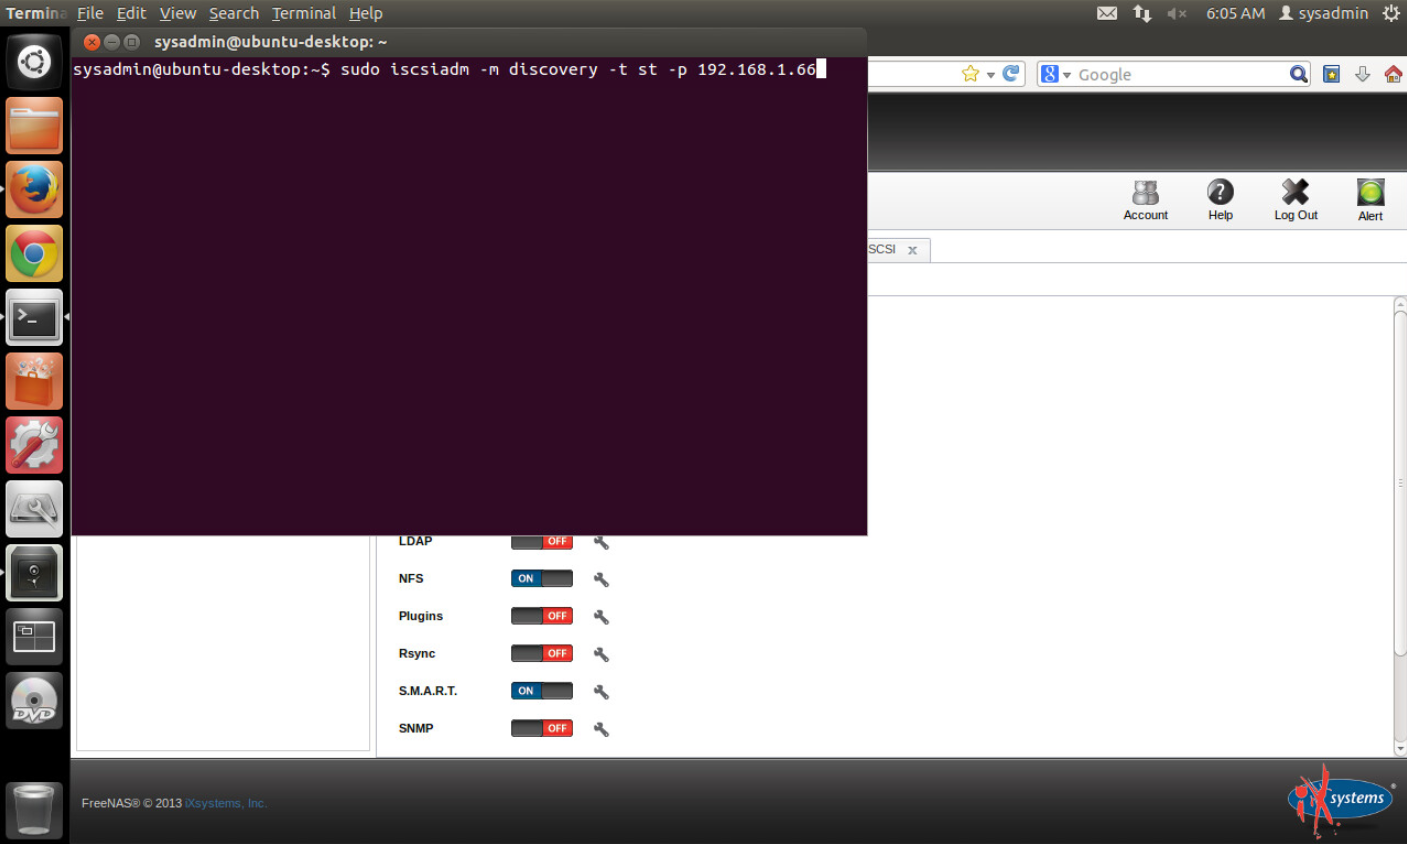
\includegraphics[width=\textwidth]{14.png}
From the screen below you can see one target found listening on port 3260. With that we copy the IQN. The IQN is basically a unique name to identify an iSCSI target \cite{iqn}.
\\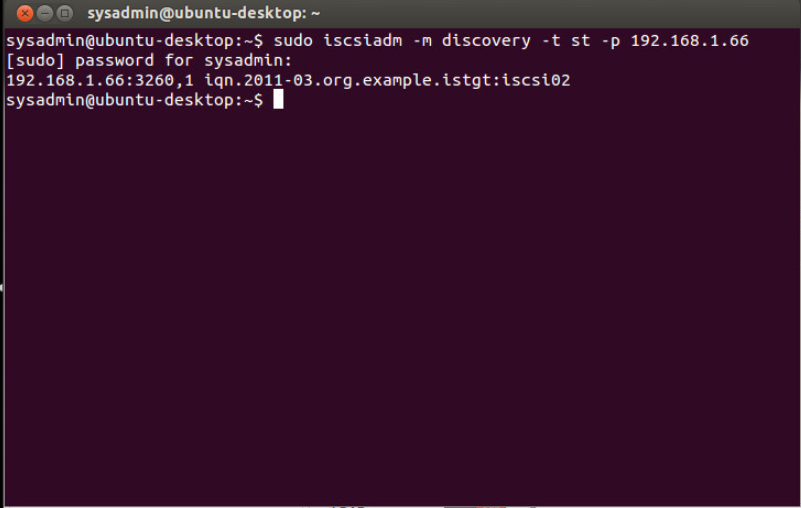
\includegraphics[width=\textwidth]{15.png}
With the IQN name copied we need to associate the host with the target node. This can be done with the following command \textit{sudo iscsiadm –-mode node –-targetname <IQN> -p 192.168.1.66 --login}. 
As can be seen from the screen below this was successful.
\\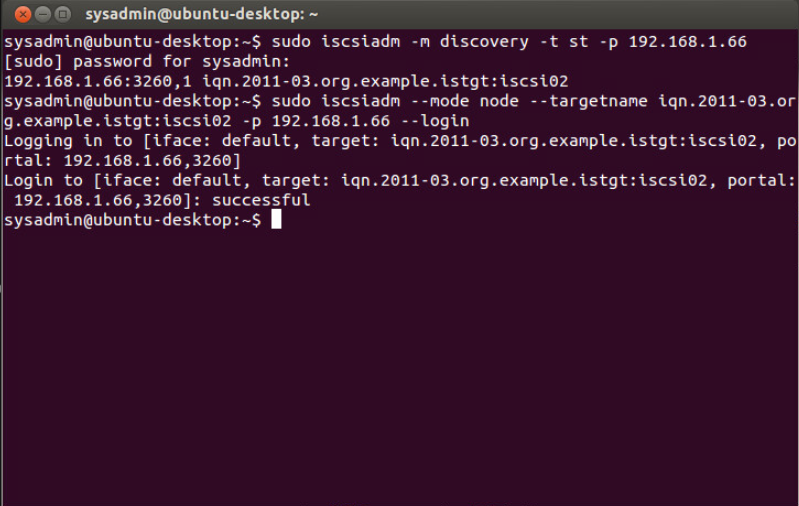
\includegraphics[width=\textwidth]{16.png}
Finally for completeness we navigate to vSphere client and go to our host VM and open a console and run the above discovery command to see if the volume is in fact available to our host clients.
\\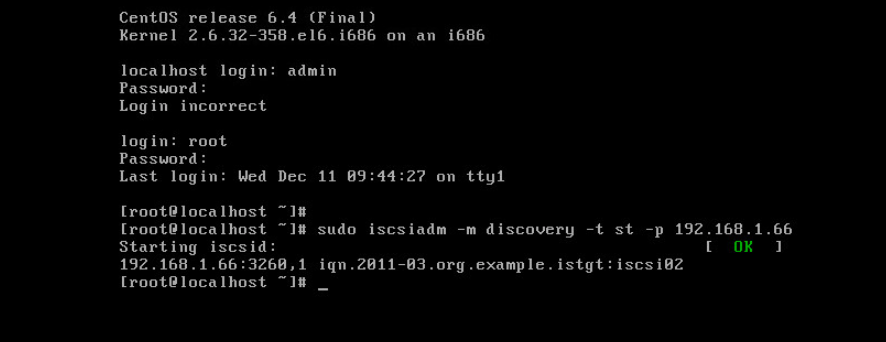
\includegraphics[width=\textwidth]{17.png}

\section{Summary}
To sum up what was covered, an iSCSI volume was configured on NAS02. The difference between file extent and device extent was explained. Security and Authentication was explained and configured on the iSCSI volume. We then associated the iSCSI volume with a host creating an iSCSI initiator, and finally using a discovery we showed that the iSCSI volume was available to the host.

\begin{thebibliography}{9}
\bibitem{iscsi} 
Margaret Rouse
\\\texttt{https://searchstorage.techtarget.com/definition/iSCSI}. 

\bibitem{raidz}
\texttt{https://blogs.oracle.com/ahl/what-is-raid-z}

\bibitem{extent}
Cormac Hogan
\\\texttt{https://blogs.vmware.com/vsphere/2012/02/vmfs-extents-are-they-bad-or-simply-misunderstood.html}

\bibitem{extent2}
\texttt{http://doc.freenas.org/11/sharing.html}

\bibitem{lun}
Carol Sliwa
\\\texttt{https://searchstorage.techtarget.com/definition/logical-unit-number}

\bibitem{CHAP}
\texttt{http://olddoc.freenas.org/index.php/ISCSI.AuthorizedAccesses}

\bibitem{iqn}
\texttt{https://pubs.vmware.com/vsphere-4-esx-vcenter/index.jsp}

\end{thebibliography}


\end{document}